% This is "sig-alternate.tex" V1.9 April 2009
% This file should be compiled with V2.4 of "sig-alternate.cls" April 2009
%
% This example file demonstrates the use of the 'sig-alternate.cls'
% V2.4 LaTeX2e document class file. It is for those submitting
% articles to ACM Conference Proceedings WHO DO NOT WISH TO
% STRICTLY ADHERE TO THE SIGS (PUBS-BOARD-ENDORSED) STYLE.
% The 'sig-alternate.cls' file will produce a similar-looking,
% albeit, 'tighter' paper resulting in, invariably, fewer pages.
%
% -------------------------------------------------------------------------
% This .tex file (and associated .cls V2.4) produces:
%       1) The Permission Statement
%       2) The Conference (location) Info information
%       3) The Copyright Line with ACM data
%       4) NO page numbers
%
% as against the acm_proc_article-sp.cls file which
% DOES NOT produce 1) thru' 3) above.
%
% Using 'sig-alternate.cls' you have control, however, from within
% the source .tex file, over both the CopyrightYear
% (defaulted to 200X) and the ACM Copyright Data
% (defaulted to X-XXXXX-XX-X/XX/XX).
% e.g.
% \CopyrightYear{2007} will cause 2007 to appear in the copyright line.
% \crdata{0-12345-67-8/90/12} will cause 0-12345-67-8/90/12 to appear in the copyright line.
%
% ----------------------------------------------------
% This .tex source is an example which *does* use
% the .bib file (from which the .bbl file % is produced).
% REMEMBER HOWEVER: After having produced the .bbl file,
% and prior to final submission, you *NEED* to 'insert'
% your .bbl file into your source .tex file so as to provide
% ONE 'self-contained' source file.
%
% ================= IF YOU HAVE QUESTIONS =======================
% Questions regarding the SIGS styles, SIGS policies and
% procedures, Conferences etc. should be sent to
% Adrienne Griscti (griscti@acm.org)
%
% Technical questions _only_ to
% Gerald Murray (murray@hq.acm.org)
% ===============================================================
%
% For tracking purposes - this is V1.9 - April 2009

\documentclass{sig-alternate}

\begin{document}
%
% --- Author Metadata here ---
%\conferenceinfo{WOODSTOCK}{'97 El Paso, Texas USA}
%\CopyrightYear{2007} % Allows default copyright year (200X) to be over-ridden - IF NEED BE.
%\crdata{0-12345-67-8/90/01}  % Allows default copyright data (0-89791-88-6/97/05) to be over-ridden - IF NEED BE.
% --- End of Author Metadata ---

\title{General Theories of Software Defect Prediction}
%\subtitle{[Extended Abstract]
\titlenote{A full version of this paper is available as
\textit{Author's Guide to Preparing ACM SIG Proceedings Using
\LaTeX$2_\epsilon$\ and BibTeX} at
\texttt{www.acm.org/eaddress.htm}}
%
% You need the command \numberofauthors to handle the 'placement
% and alignment' of the authors beneath the title.
%
% For aesthetic reasons, we recommend 'three authors at a time'
% i.e. three 'name/affiliation blocks' be placed beneath the title.
%
% NOTE: You are NOT restricted in how many 'rows' of
% "name/affiliations" may appear. We just ask that you restrict
% the number of 'columns' to three.
%
% Because of the available 'opening page real-estate'
% we ask you to refrain from putting more than six authors
% (two rows with three columns) beneath the article title.
% More than six makes the first-page appear very cluttered indeed.
%
% Use the \alignauthor commands to handle the names
% and affiliations for an 'aesthetic maximum' of six authors.
% Add names, affiliations, addresses for
% the seventh etc. author(s) as the argument for the
% \additionalauthors command.
% These 'additional authors' will be output/set for you
% without further effort on your part as the last section in
% the body of your article BEFORE References or any Appendices.

\numberofauthors{3} %  in this sample file, there are a *total*
% of EIGHT authors. SIX appear on the 'first-page' (for formatting
% reasons) and the remaining two appear in the \additionalauthors section.
%
\author{
% You can go ahead and credit any number of authors here,
% e.g. one 'row of three' or two rows (consisting of one row of three
% and a second row of one, two or three).
%
% The command \alignauthor (no curly braces needed) should
% precede each author name, affiliation/snail-mail address and
% e-mail address. Additionally, tag each line of
% affiliation/address with \affaddr, and tag the
% e-mail address with \email.
%
% 1st. author
\alignauthor
William Mensah\\
       \affaddr{WVU, Morgantown, WV}\\
       \email{wmensah@csee.wvu.edu}
% 2nd. author
\alignauthor
Adam Nelson\\
       \affaddr{WVU, Morgantown, WV}\\
       \email{anelson8@csee.wvu.edu}
% 3rd. author
\alignauthor 
Tomi Prifti\\
       \affaddr{WVU, Morgantown, WV}\\
       \email{tprifi@csee.wvu.edu}
%\and  % use '\and' if you need 'another row' of author names
% 4th. author
%\alignauthor Lawrence P. Leipuner\\
%       \affaddr{Brookhaven Laboratories}\\
%       \affaddr{Brookhaven National Lab}\\
%       \affaddr{P.O. Box 5000}\\
%       \email{lleipuner@researchlabs.org}
% 5th. author
%\alignauthor Sean Fogarty\\
%       \affaddr{NASA Ames Research Center}\\
%       \affaddr{Moffett Field}\\
%       \affaddr{California 94035}\\
%       \email{fogartys@amesres.org}
% 6th. author
%\alignauthor Charles Palmer\\
%       \affaddr{Palmer Research Laboratories}\\
%       \affaddr{8600 Datapoint Drive}\\
%       \affaddr{San Antonio, Texas 78229}\\
%       \email{cpalmer@prl.com}
}
% There's nothing stopping you putting the seventh, eighth, etc.
% author on the opening page (as the 'third row') but we ask,
% for aesthetic reasons that you place these 'additional authors'
% in the \additional authors block, viz.
%\additionalauthors{Additional authors: John Smith (The Th{\o}rv{\"a}ld Group,
%email: {\texttt{jsmith@affiliation.org}}) and Julius P.~Kumquat
%(The Kumquat Consortium, email: {\texttt{jpkumquat@consortium.net}}).}
\date{October 14 2009}
% Just remember to make sure that the TOTAL number of authors
% is the number that will appear on the first page PLUS the
% number that will appear in the \additionalauthors section.

\maketitle




\begin{abstract}

%Three different preprocessing approaches are tested on a number of datasets.
\end{abstract}

% A category with the (minimum) three required fields
\category{H.4}{Information Systems Applications}{Miscellaneous}
%A category including the fourth, optional field follows...
\category{D.2.8}{Software Engineering}{Metrics}[complexity measures, performance measures]

\section{Introduction}
By predicting defects in software systems {\em before} the deployment of that software,
it is possible to gauge not only the probable quality upon delivery, but also the maintenance effort.
Software defect prediction builds models using available company data that can then be applied in order
to predict these software faults. But in order to employ these models, a company must have
a data repository where information regarding defects from past projects are stored.
However, according to Turhan, et. al. \cite{turhan09}, few companies are applying this practice.
Turhan, et. al. claims (and we agree), that this is most likely due to a lack of local data repositories.
When this is the case, companies must use non-local data in order to build defect predictors. Thus,
it is not only important to determine how well cross-company data can be used when local data is unavailable,
but also to find the presence or absence of a general theory of software defect prediction. In other words,
in determining the existence of an empirically-derived correlation between varying defect data sets,
a statement can be made in regards to not only the stability of current defect prediction, but also the
underlying similarities of cross-company software projects. On the other hand,
if no correlation is found to exist, instability of those current predictors may suggest that further research
should be conducted in order to provide incite into the variance between projects.

%In this paper, we provide introduce recent experiments conducted by the authors of this paper in order to produce
%a general hypothesis in regards to the stability or instability of current software defect prediction theories that can be used in further analyses.

\section{Background}

The ability of an organization being able to use cross-company (CC) data
when within-company (WC) data is not available in order to build
defect predictors would be advantageous. However, it remains unclear
if this practice can yield beneficial results.

Turhan et al. conducted three experiments to rule in favor of CC data obtained from other sites, or WC data gathered locally. The conclusions of those experiments show that CC data, when applied using {\em relevancy filtering} via a k-nearest neighbor scheme. The idea behind the k-NN filter is simple; by building a training set that is homogeneous with the testing set, it is assumed that a bias in the model will be introduced. The filter works as follows: for each instance in the test set, the k nearest neighbors in the training set are chosen. Then, duplicates are removed and the remaining instances are used as the new training set. This relevancy filtering can lead to defect predictors almost as effective as WC data. Thus, as stated by Gay et. al. \cite{gay09}, ``...while local data is the preferred option, it is feasible to use imported data provided that it is selected by a relevancy filter.''

Gat et. al. confirmed Turhan et. al.'s results, but instead of implementing a nearest neighbor filter, a locally weighted scheme was used to filter the data via \cite{hallLWL}. This experiment was of significance due to the fact that Gay et. al.'s results showed not only that CC data can be used when local data is not available, but also that publicly available data such as the PROMISE \footnote{http://promisedata.org/} data.

On the other hand, \cite{zimmerman09} shows that CC data cannot be used to build accurate defect predictors. For example, in one experiment conducted by Zimmerman et. al., Firefox and Internet Explorer were used due to their domain relationship (browsers) in order to determine how well one could predict for the other. It was found that while Firefox could predict for Internet Explorer at a precision of 76.47\%, Firefox could {\em not} predict for Internet Explorer approaching the same precision (4.12\%). However, this experiment did not utilize any form of relevancy filtering, so it is unknown how the two data sets would react to predicting for one another under these circumstances.

If CC data, when filtered, can be used in order to predict defects, we are left to assume that this is due to the fact that the data sets share some innate similarities of their metrics. But if it is found conclusively that CC data cannot most generally build good defect predictors, we are to conclude that other measures must be taken in either the collection of the WC data, or for more research in the further filtering of CC data.


\section{Finding Generality}
In an ideal situation a company would have large amount of data from a software project that can be used to build models that can predict defects for
future releases of the software. In practice however training data from within company is not available in most of the cases. Using data from other projects or other companies is the only option to build prediction models. An ideal model will be able to predict software defect of a project even if trained on data obtained outside the company. Zimmerman et. al in their paper
try to asess the extent that cross-project data can be used to predict defects and what kind of software systems are good for cross-predictors. Their results
show that simply using projects in the same domain does not work to build accurate prediction models. In our work we are trying to find generality
between cross data projects following a different approach based on prism rule learner.

\section{The Experiment}


\subsection{Preparing the Data}
The data we are using for to test our is extracted from two very different companies: NASA and SoftLab (a turkish software company). The data sets are shown below.
\\NASA Datasets
\begin{itemize}
\item{ KC1. Storage Management for ground data }
\item{PC1. Flight Software for each orbiting satellite}
\item{KC2 Storage management for ground data}
\item{CM1} Spacecraft Instrument
\\Turkish Datasets
\item {AR4} embedded controller for dish washer
\item{AR3} Embedded controller for washing machine
\item{AR5} Embedded controller for refrigerator
\end{itemize}
We employed a number of preprocessing techniques to prepare the original data before applying our learner to it. These include:

\begin{itemize}
\item{Discretization}
\\Splitting each data set randomly into {\em 10} bins (by default)
\item{Feature Subset Selection}
\\Sample bias via {\em B-Square} whereby each column in the data set is ranked by some criteria and the top n columns are maintained and used for the experiment because they are more likely to have a stronger influence on the results.
\end{itemize}
Why are all these preprocessing techniques necessary? Why not use the data in its raw form? When it comes to data mining, real world data is considered by most software engineers as {\em dirty}. This is because the data could be incomplete in that it could be missing some attributes or attribute values or it could simply consist of only aggregated values. Moreover, the data could be inconsistent, and could also contain errors and outliers. Preprocessing transforms the data into a format that will be more easily and effectively processed.


\subsubsection{Discretization technique}
We discretized the data using Equal Interval Width (10 bins). This method falls under the unsupervised discretization methods class. Equal bin length is a global techinque which replaces each value by the identifier of the bin. The range of values is divided into k equally sized bins where k is a parameter manually supplied for the purpose of our experiment. For each attribute the maximum and the minimum are recorded and the range is divided into 10 equal bins. Equal in frequency is easy and straightforward to implement however does not guarantee that the instances falling in each bin will be of the same frequency. It makes no use of the instance class and is thus an unsupervized discretization method. Equal Bin Length is a global discretization method since it produces a mesh over the entire n-dimensional instance space. Other discretization techniques such as Equal Frequency Bin or Feyyad Irani could be used as a discretization technique. Research on the field shows that discretization increases the accuracy of the learner however there is no significant increase in performance in using a specific discretizer over the other \cite {dough95}.

\subsubsection{Merging Cross-Company Data}

In order to create a large, unified data set from which attributes could be selected, the data sets used in this experiment were merged. The intuition behind this was that if final rules generated from the experiment were to reflect upon the similarities (generalities) in cross-company data, those rules should thus be constructed from portions of a larger, unified pool of data. The results from the experiment should, in theory, provide the ability to predict accurately the defects in cross-company data if a general theory of software defect prediction in fact exists.

The merged data used in the experiment, as seen above, resulted in 5000 instances, on which attribute selection, row pruning and rule generation was used.

\subsubsection{Feature Subset Selection via B-Square}

B-Square served as the sole feature subset selection (FSS) method employed to assist us in modelling the data based on not only the most important attributes, but also to decrease the overall runtimes of experimentation using the data. The pseudocode for B-Square is outlined as follows:

\begin{centering}
\begin{enumerate}
\item Replace each class symbol with a utility score: True = 1, False = 0.
\item Sort instances by that score and divide them using N=20\%-chops.
\item Label all the rows in bin=1 (20\%) "best" and the remaining (80\%) "rest".
\item Collect the frequencies of ranges in best/rest.
\item Sort each range (r) by b^^2/(b+r) where
\item b = freq(r in Best) / SizeOfBest
\item r = freq(r in Rest) / SizeOfRest
\item Sort each attribute by the median score of b2/(b+r).
\item Reject attributes with less than X\% of the max. median score. 
\end{enumerate}
\end{centering}

The top five attributes were selected using B-Square from the merged data set, and then this data set was reconstructed using only those attributes. This decreased the columns of the data significantly, allowing more lengthy experiments to be conducted.

\subsubsection{Slice Generation}

The reconstructed, attribute-reduced data was then randomly placed into 50 bins by iteratively filling each bin with randomly selected instances from the entire data set. Each bin was designated as a "slice" in our experiment.

\subsubsection{Row Pruning via K-means}

In order to remove potential outliers from the data, each slice was clustered using a naive K-means clustering algorithm. K-means clustering groups similar instances together iteratively by finding a cluster's center of mass. K-means works as follows:

\begin{centering}
\begin{enumerate}
\item{Select initial {\em K} centroids at random;}
\item{Assign each incoming point to its nearest centroid;}
\item{Adjusts each cluster's centroid to the mean of each cluster;}
\item{Repeat steps 2 and 3 until the centroids in all clusters stop moving by a noteworthy amount}
\end{enumerate}
\end{centering}

Twelve clusters were generated from each slice, and the largest cluster

\subsection{Learners}
\subsubsection{PRISM}
One of the learners we used in our experiment was {\em PRISM}. Its algorithm was first introduced by Cendrowska and its aim is to induce molecular classification rules directly from the training set.

Prism uses the '{\em take the first rule that fires}' conflict resolution strategy when the resulting rules are applied to unseen data. Simply speaking, it identifies a rule that covers many instances in a given class, separates out the covered instances and continues with the remainder of the data.

When working with the Prism learner, we first calculate the probability that class = i for each attribute / value pair. After that we select the pair with the largest probability and create a subset of the training set compromising all the instances with the selected attribute / value combination (for all classifications). We then repeat the previous steps for this subset until a subset is reached that contains only instances of class i. The induced rule is then the conjunction of all the attribute / value pairs selected. Finally, we remove all instances covered by this rule from the training set.


The pseudo-code for the Prism algorithm can be outlined as follows:
\begin{verbatim}
For each class C
Initialize E to the instance set
While E contains instances in class C
  Create a rule R with an empty left-hand
  side that predicts class C
  Until R is perfect 
  (or there are no more attributes to use) do
For each attribute A not mentioned in R, 
and each value v,
  Consider adding the condition A = v 
  to the left-hand side of R
Select A and v to maximize the accuracy p/t
Add A = v to R
Remove the instances covered by R from E
\end{verbatim}

Both the Turkish data and data from NASA comprised of True / False classes, and also had quite a number of attributes in common so we figured Prism was a good option to explore, especially when it comes to cross-project defect prediction. The effect of using Prism on our datasets is analysed and discussed in our {\em Results} section.


\subsection{Experiment 1: Prism}

The Prism learner, described in section 4.2.1, was modeled by training on the training set and applying the ruleset generated to the test set. In general, the experiment with Prism involved combining all the datasets into one gigantic datasets consisting of over 5700 instances which were later randomized into 50 slices. For each slice, K-means was applied and the cluster with the most number of instances was selected to be used in place of the slice sinceits much smaller and contains more relevant data as determined by the K-means algorithm. After K-means had been run on all 50 slices, 10% of the clusters obtained were allocated to be used as testing and the remaining 90% for training the learner.

Once preparation of the data had been completed, our experiment entailed iterating through each dataset in the training set and generating new rules, applying those rules to the test set and comparing the results of the probability of defect (pd) to that of the Rulest when applied to the test set as well. The pseudocode describing the algorithm is outlined as follows


\begin{verbatim}
for each slice s do
if Better (ruleset, s)
  continue
else
  ruleset = Rebuild (s, ruleset)
  if !Better (s, ruleset) then
    ruleset = s
    end if
end for

procedure Better (s, ruleset)
if pd(ruleset) > pd(s)
    return true
return false

\end{verbatim}

With reference the algorithm, whenever the pd of the Ruleset is better than that of the current slice, iteration proceeds to the next slice; otherwise, a new Ruleset is generated by rebuilding or simply merging the two datasets. Once this is done, the current slice is given another chance to obtain apd better than that of the Ruleset. If this turns out to be the case, data from the Ruleset is replaced with that of the slice and the iteration is carried on. This is done because the slice's data is much smaller than theRuleset's and is deemed a better defect predictor.

The operation described above was repeated 500 times and each time, besides the first iteration, the Ruleset from the previous iteration was maintained. While this time-expensive operation was carried out, changes in the Ruleset was tracked. A best case scenario is where theRulset never changes throughout all 500 runs and a worst case scenario is where the Ruleset changes everytime. The former would result in a consistent horizontal line when graphed whereas the latter would result in a straight diagonal line. The results of our experiment is discussed in the next section.

\subsection{Experiment 2: Naive Bayes}

The Bayes classifier is a simple statistical-based learning scheme. For this experiment, it was used as a secondary learner, in order to compare its results to that of Prism, our primary learner. Before the experiment could be conducted, the data had to be preprocessed as described in section 4.1 and the train and test sets were derived using the same approach described in the previous section for Prism. However, in this experiment, the generation of rules was omitted. Naive Bayes simply trained on the training set obtained after applying K-means on the slices and then tested on.


\section{Results}
The cumulative graph above shows the number of times that Ruleset loses when compared to a new set of rules as we iterate through the training set. The graph shows clearly that our learner is {\em not} converging to an optimal set of rules that willalways win when compared to new set of rules.

The following PD and PF values represent results obtained by training on data set A, and attempting to predict on data set B. It can be shown that neither learner performs well predicting cross company defects.

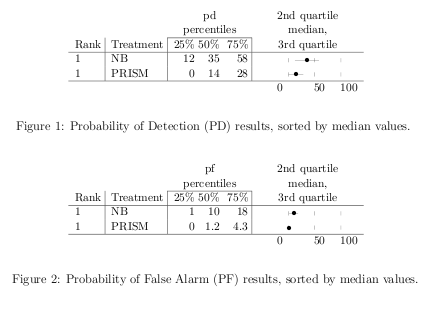
\includegraphics[width=243px, height=149px]{pd.png}
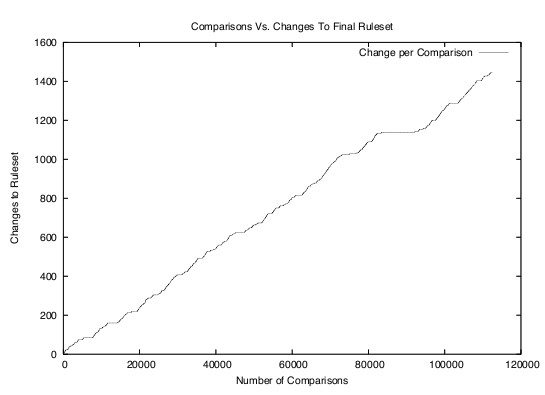
\includegraphics[width=90mm, height=60mm]{iter.png}

\caption{Comparison vs. Changes to Final Ruleset}


\section{Related Work}
This project is inspired by the Cross-project Defect Prediction work conducted by Thomas Zimmerman et. al. who claimed that software defect prediction works well whenever there is sufficient data to train any models and that in the case where data is insufficient, cross-project defect prediction suffices\cite{zimmerman09}. In their experiment, they ran 622 cross-project predictions for 12 real-world applications including Microsoft's Internet Explorer and Mozilla Foundation's Firefox web browser, and their results indicated that simply using models from projects in the same domain or with the same process does not lead to accurate predictions. With respect to the experiments they conducted, they learned that Firefox could predict defects in Internet Explorer but not vice versa and they succumbed to the conclusion that this is so because Firefox has more files than Internet Explorer has binaries and that the probability of a software with more data is more likely to predict defects in software with relatively less amount of data or modules.

Their study led to conclusions that some attributes were less significant than others which is somewhat obvious but also lead to questions such as why defect-prediction is not transivitve. As in, with regards to the experiments they conducted, File system predicted defects in Printing and Printing predicted Clustering but File system did not predict Clustering.

%\newpage
\section{Conclusions}
The results from the experiment shows that our learner fails to find generality in the data.
Prism fails to converge to a rule set that generalizes through all datasets partitions. According to our
approach and experiments, the prediction methods lack evidence of generality in cross-over company data.
This evidence is supported by the divergence of rules and the low probabilities of detection. Based on
this results, PRISM is not a suitable learner for predicting software defects on the data of this nature.
Our results are similar to those of  Zimmerman et. al in that they fail to show evidence of generality in 
cross-company defect prediction. On the other hand existing research in the field, such as that of Turan et. al, hints
at generality in cross-company data. This highlights the importance of requiring confirmation in our experimental results.  

\section{Future Work}
An alternate approach worth exploring that could shed some light on this experiment is to split up each slice into train and test sets after clustering rather than taking the largest cluster. This method allows for the realization of generality in the case where the learner is able to predict defects for each test fairly well provided some treshhold has been given. Futhermore, unless pressed for time, more runs could be conducted, say 1000 with hopes of finding a converging graph. Moreover, different preprocessing techniques such as microsampling and other learners besides Naive Bayes and Prism could be exploitedto achieve results that could be compared to that of our experiment. 

\section{Acknowledgments}
We will like to thank Dr. Menzies, Associate Professor (Computer Science & Electrical Engineering) at West Virginia University, for his assistance in the acquisition of the datasets used for the experiment described in the context of this paper and enlightening us with the tools and techniques that were used. 

%
% The following two commands are all you need in the
% initial runs of your .tex file to
% produce the bibliography for the citations in your paper.
\bibliographystyle{abbrv}
\bibliography{refs} % sigproc.bib is the name of the Bibliography in this case
% You must have a proper ".bib" file
% and remember to run:
% latex bibtex latex latex
% to resolve all references
%
% ACM needs 'a single self-contained file'!
%
%APPENDICES are optional
%\balancecolumns

\end{document}   
